%%% LaTeX Template: Article/Thesis/etc. with colored headings and special fonts
%%%
%%% Source: http://www.howtotex.com/
%%% Feel free to distribute this template, but please keep to referal to http://www.howtotex.com/ here.
%%% February 2011
%%%
%%% Modified October 2015 by CDM

%%%  Preamble
\documentclass[11pt,letterpaper]{article}
\usepackage[margin=1.0in]{geometry}
\usepackage[T1]{fontenc}
\usepackage[bitstream-charter]{mathdesign}
\usepackage[latin1]{inputenc}					
\usepackage{amsmath}						
\usepackage{xcolor}
\usepackage{cite}
\usepackage{hyphenat}
\usepackage{graphicx}
\usepackage{float}
\usepackage{subfigure}
\usepackage{sectsty}
\usepackage[compact]{titlesec} 
\usepackage[tablegrid]{vhistory}
\allsectionsfont{\color{accentcolor}\scshape\selectfont}

%%% Definitions
\definecolor{accentcolor}{rgb}{0.0,0.0,0.5} 
\newcommand{\teamname}{Smart Hospital Dev Team}
\newcommand{\productname}{S.H. Management Tool}
\newcommand{\coursename}{CSE 4316: Senior Design I}
\newcommand{\semester}{Fall 2016}
\newcommand{\docname}{System Requirements Specification}
\newcommand{\department}{Department of Computer Science \& Engineering}
\newcommand{\university}{The University of Texas at Arlington}
\newcommand{\authors}{Allison Johnsgard \\ Edward Fankhauser \\ Narayan Rimal \\ Neelim Haider \\ Victor Garcia}

%%% Headers and footers
\usepackage{fancyhdr}
	\pagestyle{fancy}						% Enabling the custom headers/footers
\usepackage{lastpage}	
	% Header (empty)
	\lhead{}
	\chead{}
	\rhead{}
	% Footer
	\lfoot{\footnotesize \teamname \ - \semester}
	\cfoot{}
	\rfoot{\footnotesize page \thepage\ of \pageref{LastPage}}	% "Page 1 of 2"
	\renewcommand{\headrulewidth}{0.0pt}
	\renewcommand{\footrulewidth}{0.4pt}

%%% Change the abstract environment
\usepackage[runin]{abstract}			% runin option for a run-in title
%\setlength\absleftindent{30pt}			% left margin
%\setlength\absrightindent{30pt}		% right margin
\abslabeldelim{\quad}	
\setlength{\abstitleskip}{-10pt}
\renewcommand{\abstractname}{}
\renewcommand{\abstracttextfont}{\color{accentcolor} \small \slshape}	% slanted text

%%% Start of the document
\begin{document}

%%% Cover sheet
{\centering \huge \color{accentcolor} \sc \textbf{\department \\ \university} \par}
\vspace{1 in}
{\centering \huge \color{accentcolor} \sc \textbf{\docname \\ \coursename \\ \semester} \par}
\vspace{0.5 in}
\begin{figure}[h!]
	\centering
   	
\includegraphics[width=0.60\textwidth]{images/ribbonbanner}
\end{figure}
\vspace{0.5 in}
{\centering \huge \color{accentcolor} \sc \textbf{\teamname \\ \productname} \par}
\vspace{0.5 in}
{\centering \large \sc \textbf{\authors} \par}
\newpage


%\vspace{1 in}
%\centerline{January 13th, 2012}
%\newpage

%%% Revision History
\begin{versionhistory}
  	\vhEntry{0.0.1}{07.15.2016}{EF}{document creation}
  	\vhEntry{0.0.2}{10.05.2015}{AJ, EF, NR, NH, VG}{Turn-in candidate 1}
  	\vhEntry{0.1.0}{10.12.2015}{EF}{First Turn-in}
\end{versionhistory}
\newpage

%%% Table of contents
\setcounter{tocdepth}{2}
\tableofcontents
\newpage

%%% List of figures and tables (optional)
\listoffigures
%\listoftables
\newpage

\section{Product Concept}
This sections describes the purpose, use, and intended user audience for the Smart Hospital Management Tool. The Smart Hospital Management Tool that performs managing the inventory and keeps track of employees' schedules. The Smart Hospital faculty and students will be able to schedule simulations, check out tools, clock their worked hours, and iventory management.

\subsection{Purpose and Use}
The Smart Hospital Management Tool is a web-base software application to help the Smart Hospital manage their inventory, employee schedules, time, generated reports, and other factors. The Smart Hospital faculty and students will access the Smart Hospital Management Tool through a web browser and schedule simulations.

\subsection{Intended Audience}
The Smart Hospital Management Tool will be used by the Smart Hospital faulty, graduate students, and undergraduate students. In the future, other colleges may wish to incorporate the software which will be freely available.

\begin{figure}[h!]
	\centering
   	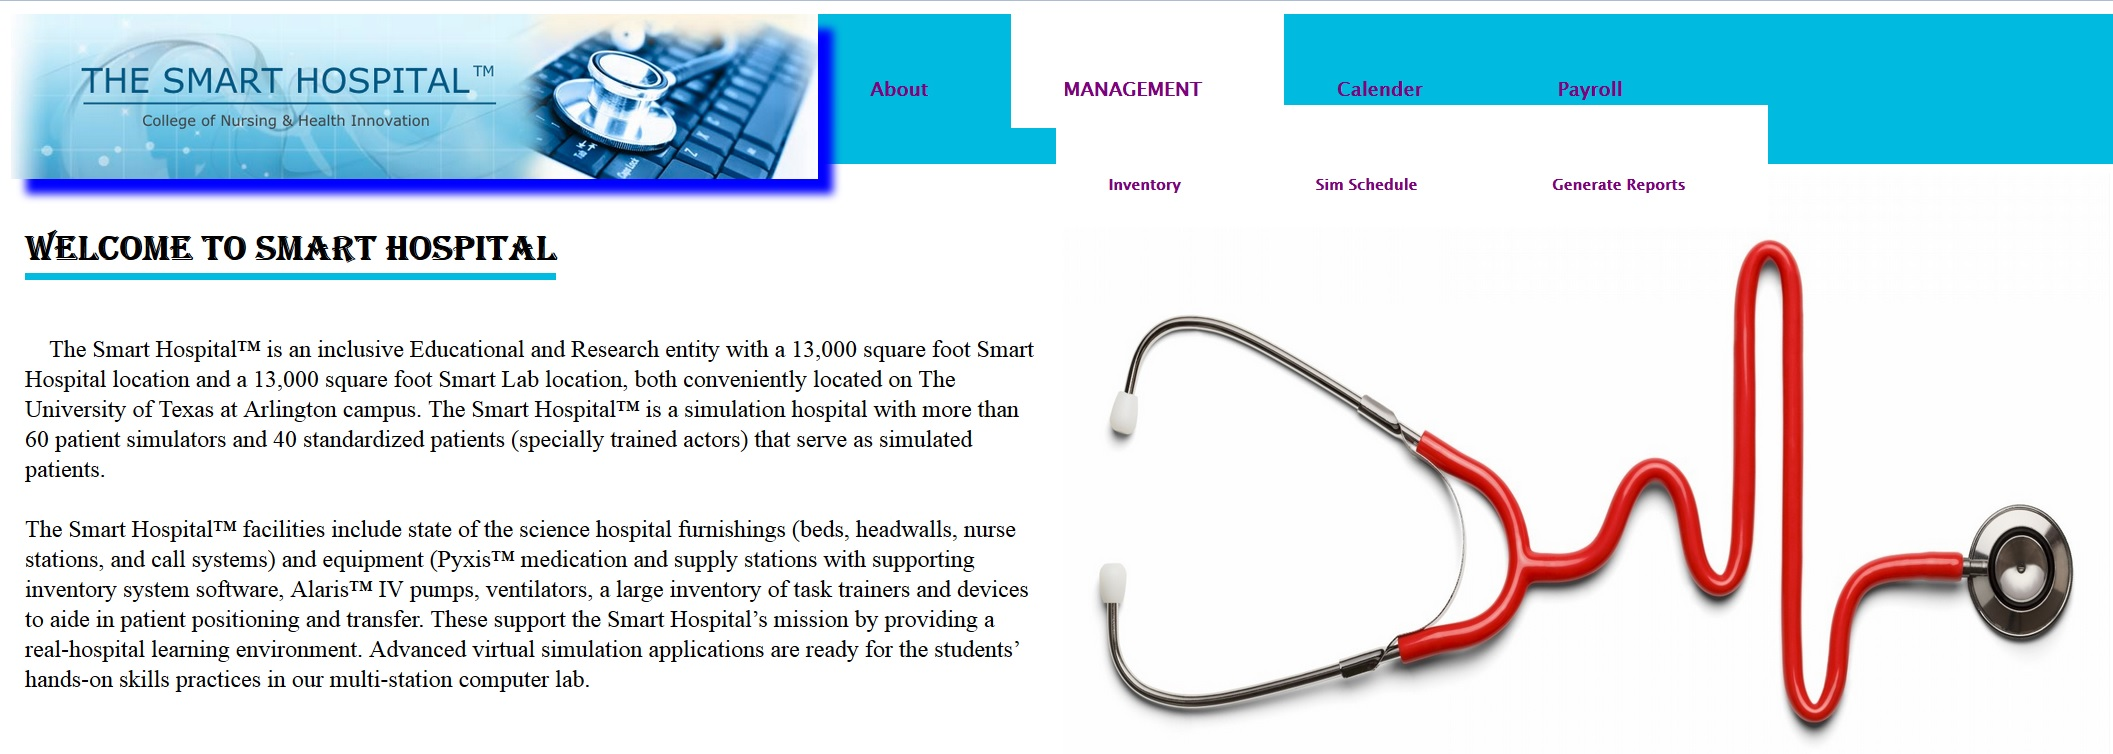
\includegraphics[width=0.60\textwidth]{images/concept_screenshot_1}
    \caption{X conceptual drawing}
\end{figure}

\newpage
\section{Product Description}
This section provides a description of your product and defines it's primary features and functions. The purpose is to give the document reader/reviewer enough information about the product to allow them to easily follow the specification of requirements found in the remainder of the document. Your header for this section should introduce the section with a brief statement such as: "This section provides the reader with an overview of X. The primary operational aspects of the product, from the perspective of end users, maintainers and administrators, are defined here. The key features and functions found in the product, as well as critical user interactions and user interfaces are described in detail." Using words, and pictures or graphics where possible, specify the following:

\subsection{Features \& Functions}
What the product does and does not do. Specify in words what it looks like, referring to a conceptual diagram/graphic (Figure X).  Define the principle parts/components of the product. Specify the elements in the diagram/graphic that are part(s) of this product as well as any associated external elements (e.g., the Internet, an external web server, a GPS satellite, etc.)

\subsection{External Inputs \& Outputs}
Describe critical external data flows. What does your product require/expect to receive from end users or external systems (inputs), and what is expected to be created by your product for consumption by end users or external systems (outputs)? In other words, specify here all data/information to flow into and out of your systems. A table works best here, with rows for each critical data element, and columns for name, description and use.

\subsection{Product Interfaces}
Specify what all operational (visible) interfaces look like to your end-user, administrator, maintainer, etc. Show sample/mocked-up screen shots, graphics of buttons, panels, etc. Refer to the critical external inputs and outputs described in the paragraph above.

\newpage
\section{Customer Requirements}
Include a header paragraph specific to your product here. Customer requirements are those required features and functions specified for and by the intended audience for this product. This section establishes, clearly and concisely, the "look and feel" of the product, what each potential end-user should expect the product do and/or not do. Each requirement specified in this section is associated with a specific customer need that will be satisfied. In general Customer Requirements are the directly observable features and functions of the product that will be encountered by its users. Requirements specified in this section are created with, and must not be changed without, specific agreement of the intended customer/user/sponsor.

\subsection{Requirement Name}
\subsubsection{Description}
A detailed description of the feature/function that satisfies the requirement. For example: \textit{The box will be slate blue. This specific color is required in order to ensure that the box matches other similar boxes in the Box Systems Premium line of products. Slate blue is specified as \#007FFF, using six-digit hexadecimal color specification.} It is acceptable and advisable to include drawings/graphics in the description if it aids understanding of the requirement.
\subsubsection{Source}
The source of the requirement (e.g. customer, sponsor, specified team member (by name), federal regulation, local laws, CSE Senior Design project specifications, etc.)
\subsubsection{Constraints}
A detailed description of constraints on satisfying the requirement (e.g. one such constraint might be: \textit{The specified color must be commercially available in paint capable of adhering to the material of which the box is manufactured. (See customer requirement 3.x for production material specification.)}
\subsubsection{Standards}
A detailed description of any specific standards that apply to this requirement (e.g. \textit{NSTM standard xx.xxx.x. color specifications \cite{Rubin2012}}.)
\subsubsection{Priority}
The priority of this requirement relative to other specified requirements. Use the following priorities:
\begin{itemize}
\item Critical (must have or product is a failure)
\item High (very important to customer acceptance, desirability)
\item Moderate (should have for proper product functionality);
\item Low (nice to have, will include if time/resource permits)
\item Future (not feasible in this version of the product, but should be considered for a future release).
\end{itemize}

\subsection{Requirement Name}
\subsubsection{Description}
Detailed requirement description...
\subsubsection{Source}
Source
\subsubsection{Constraints}
Detailed description of applicable constraints...
\subsubsection{Standards}
List of applicable standards
\subsubsection{Priority}
Priority

\newpage
\section{Packaging Requirements}
Include a header paragraph here. Packaging requirements are those requirements that identify how the delivered product will be packaged for delivery to the end-user; or how it will "look" when finished and delivered. For example, you might specify that the software required for operation will be pre-loaded on the hard drive, delivered on CD/DVD, or available via download. Software might be customer installable, or not, etc. Hardware components could be all in a single package, provided as a "bag of parts" to be assembled/installed by the user, painted a certain color, logos affixed, etc. Care should be taken not to duplicate requirements found in other sections of this document.

\subsection{Source Code Avaliability}
\subsubsection{Description}
The source code shall be available on the SmartHospital gitHub respository.
\subsubsection{Source}
Dev Team
\subsubsection{Standards}
N/A
\subsubsection{Priority}
Moderate
\newpage
\section{Performance Requirements}
The performance section relates to how fast the website will respond to user input, queries, and page loads.

\subsection{Database Load}
\subsubsection{Description}
The database shall load in under 1 second.
\subsubsection{Source}
Dev Team
\subsubsection{Constraints}
Connection Speed
\subsubsection{Priority}
Low

\subsection{Inventory List Load}
\subsubsection{Description}
The inventory list shall load in under 1 second on each new search query.
\subsubsection{Source}
Dev Team
\subsubsection{Constraints}
Connection Speed
\subsubsection{Priority}
Low

\subsection{Calendar Display Load}
\subsubsection{Description}
The Calendar shall load in under 1 second on each view.
\subsubsection{Source}
Dev Team
\subsubsection{Constraints}
Connection Speed
\subsubsection{Priority}
Low

\subsection{UI Adjustment Speed}
\subsubsection{Description}
The UI shall adjust to resizing as the website borders are moved.
\subsubsection{Source}
Dev Team
\subsubsection{Constraints}
Connection Speed
\subsubsection{Priority}
Low
\newpage
\section{Safety Requirements}
This section covers safety features that the Smart Hospital Management Tools will implement.

\subsection{Location Aware Clock}
\subsubsection{Description}
The website shall allow clock ins to be limited to specific location.
\subsubsection{Source}
Stone Kim
\subsubsection{Standards}
N/A
\subsubsection{Priority}
Moderate

\subsection{Password Recovery}
\subsubsection{Description}
The website shall allow the registered users to recover their password.
\subsubsection{Source}
Dev Team
\subsubsection{Standards}
N/A
\subsubsection{Priority}
High

\subsection{Password Encryption}
\subsubsection{Description}
The website shall encrypt passwords that are saved to the database.
\subsubsection{Source}
Dev Team
\subsubsection{Standards}
N/A
\subsubsection{Priority}
Low

\newpage
\section{Maintenance \& Support Requirements}
This sections describes how the product will be maintained. Dev Team will provide support until May 2017. After this time, the maintenance will be up to the Smart Hospital faculty. Also, a user manual will be provided to the Smart Hospital faculty in order for the faculty to be able to operate the software.

\subsection{Maintenance}
\subsubsection{Description}
The team will provide short term maintanence up until May 2017.
\subsubsection{Source}
Dev Team
\subsubsection{Priority}
Future

\subsection{User Manual}
\subsubsection{Description}
The team shall provide a manual covering how to do certain things such as adding inventory items.
\subsubsection{Source}
Dev Team
\subsubsection{Priority}
Moderate
\newpage
\section{Other Requirements}
This section describes requirements that did not fit into the other categories.


\subsection{Personel Database}
\subsubsection{Description}
The website shall contain a database of students and faculty associated with the Smart Hospital.
\subsubsection{Source}
Dev Team
\subsubsection{Standards}
N/A
\subsubsection{Priority}
High

\subsection{Alternate Sign-in}
\subsubsection{Description}
The website shall allow creation of website based accounts.
\subsubsection{Source}
Dev Team
\subsubsection{Standards}
N/A
\subsubsection{Priority}
Critical



\newpage
\section{Future Items}
In this last section, you will reiterate all requirements that are listed as priority 5. This is repetitive, but necessary as a concise statement of features/functions that were considered/discussed and documented herein, but will NOT be addressed in the prototype version of the product due to constraints of budget, time, skills, technology, feasibility analysis, etc. Use the following format for this section.

\subsection{UTA Single Sign-on}
\subsubsection{Description}
The website shall incorporate the UTA single sign-on system with the log in system for the Smart Hospital website.
\subsubsection{Source}
Soohyun Kim
\subsubsection{Constraints}
OIT Needs to allow access
\subsubsection{Standards}
N/A
\subsubsection{Priority}
Future

\subsection{Room Designation}
\subsubsection{Description}
The system shall display the location of available rooms for a user wanting to schedule a room.
\subsubsection{Source}
Soohyun Kim
\subsubsection{Standards}
N/A
\subsubsection{Priority}
Future
\newpage

%%% References
\bibliographystyle{plain}
\bibliographystyle{reference/IEEEtran_custom}
\bibliography{reference/refs}{}

\end{document}